\documentclass[12pt]{article}
\usepackage{amsmath, graphicx, caption}
\usepackage{amsthm}
\usepackage{amsfonts, xcolor, physics}
\usepackage{amssymb}
\usepackage{mathrsfs}
\usepackage[T1]{fontenc} % for \symbol{92} 
\usepackage{comment}


\addtolength{\oddsidemargin}{-1in}
\addtolength{\evensidemargin}{-1in}
\addtolength{\textwidth}{1.75in}
\addtolength{\topmargin}{-1in}
\addtolength{\textheight}{1.75in}
\newcommand{\contra}{$\rightarrow\leftarrow$}
\newcommand{\tb}{  \textbackslash  }
\newcommand{\bj}{\ \Longleftrightarrow \ }

%bailey meche
\begin{document}
%bailey meche
	\begin{center}
		Assignment 3: Critical points and approximation\\
        MACSS 33000 1 \\
		Due Tuesday, August 28 \\
        %Bailey Meche
	\end{center}
 
\section{Sketch a function}
Sketch the graph of a function (any function you like, no need to specify a functional form) that is:
\begin{enumerate}
    \item Continuous on $[0,3]$ and has the following properties: an absolute minimum at 0, an absolute maximum at 3, a local maximum at 1 and a local minimum at 2.
    \item Do the same for another function with the following properties: 2 is a critical number (i.e. $f'(x) = 0$ or $f'(x)$ is undefined), but there is no local minimum and no local maximum.
\end{enumerate}
Solution
\begin{enumerate}
    \item $f(x)=\frac{1}{5}x^{5}-\frac{3.2}{4}x^{4}+\frac{2.5}{5}x^{3}+2x$

\begin{figure}[h!]
\centering
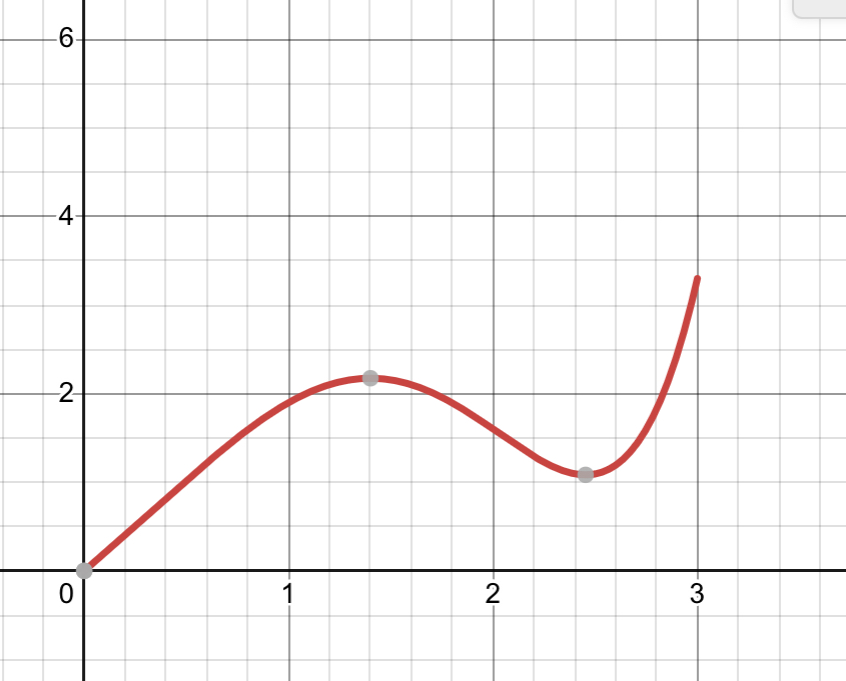
\includegraphics[height=6cm]{G1.1.jpeg}
\captionsetup{labelformat=empty}
%\caption{2. $y = f(x)$}
\end{figure}

    \item $f(x)=\left(x-2\right)^{\frac{1}{5}}+2$


\begin{figure}[h!]
\centering
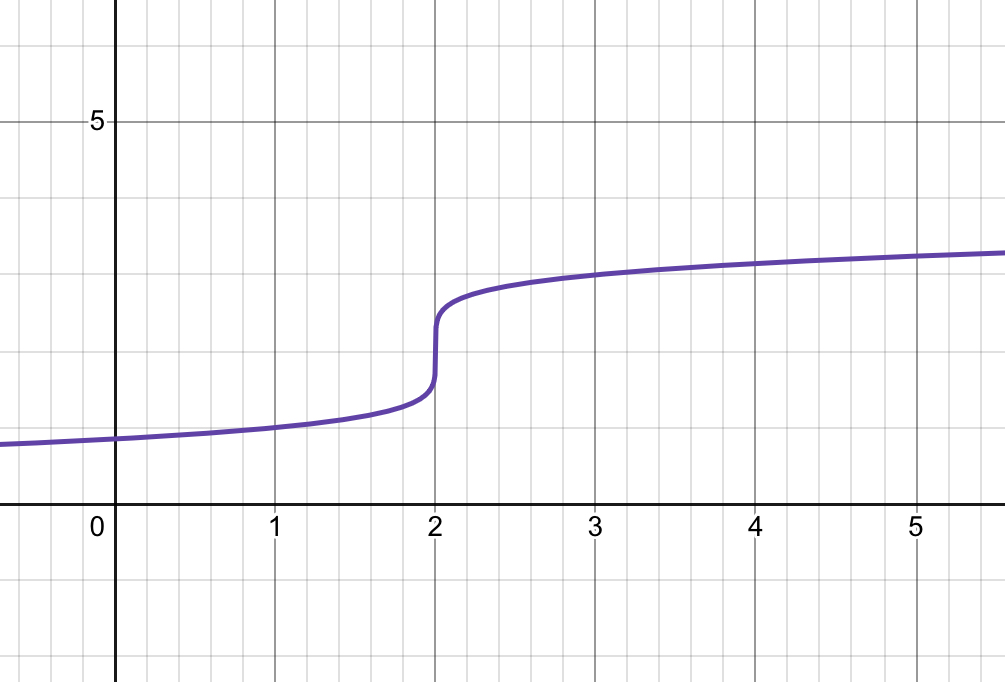
\includegraphics[height=6cm]{G1.2.jpeg}
\captionsetup{labelformat=empty}
%\caption{2. $y = f(x)$}
\end{figure}

\end{enumerate}

\section{Find the critical values}
Find the critical values of these functions
\begin{enumerate}
    \item $f(x)= 5x^{3/2} -4x$
    \item $s(t) = 3t^4 + 4t^3 - 6t^2$
    \item $f(r) = \frac{r}{r^2+1}$
    \item $h(x) = x\log(x)$
\end{enumerate}
Solution
\begin{enumerate}
    \item $f'(x)= 5\cdot \frac{3}{2}x^{1/2} -4$
    
    For $f'(x)=0$, 
    \begin{align*}
            5\cdot \frac{3}{2}x^{1/2} -4 &=0
            \\ x^{1/2} &= \frac{8}{15}
            \\ x &= \pm \sqrt{\frac{8}{15}} = 2\sqrt{\frac{2}{15}}
            \\ x &= \pm \frac{2\sqrt{30}}{15} = \text{ critical values of } f(x)
    \end{align*}
    \item $s'(t) = 12t^3 + 12t^2 - 12t$

    For $s'(t)=0$,
    \begin{align*}
        12t^3 + 12t^2 - 12t &= 0
        \\ 12t(t^2 +t -1) &=0
        \\ t &= 0, \frac{-1 \pm \sqrt{5}}{2}
    \end{align*}
    \item $f'(r) = \frac{1 - r^2}{(r^2+1)^2}$

    For $f'(r)=0$,
    \begin{align*}
        \frac{1 - r^2}{(r^2+1)^2} &=0
        \\ 1-r^2 &= 0 
        \\ -(r-1)(r+1) &=0
        \\ r&= \pm 1
    \end{align*}
    \item $h'(x) = \log(x)+ 1$

    For $h'(x)=0$,
    \begin{align*}
        \log(x)+1&=0
        \\ x &= e^{-1}=\frac{1}{e}
    \end{align*}
\end{enumerate}

\section{Find the absolute minimum/maximum values}
Find the absolute minimum and absolute maximum values of the functions on the given interval
\begin{enumerate}
    \item $f(x) = 3x^2 -12x + 5$ s.t. $x\in [0,3]$
    \item $f(t) = t\sqrt{4-t^2}$ s.t. $ t \in [-1,4]$
    \item $s(x) = x-\ln(x)$ s.t. $x \in [\frac{1}{2},2]$
    \item $h(p) = 1-e^{-p}$ s.t. $p \in [0,1000]$
\end{enumerate}
Solution
\begin{enumerate}
    \item $f'(x) = 6x -12$
    
    Finding the critical points, we find $x=2$. Since $f''(x)=6>0$, the point $(2,-7)$ is an absolute minimum on the interval $[0,3]$. To find the absolute maximum, we test the endpoints to find $(0,5).$
    
    \item $f'(t) =\sqrt{4-t^2} -t^2(4-t^2)^{-\frac{1}{2}}$

    Finding the critical points, 
    \begin{align*}
        f'(t) = \sqrt{4-t^2} -t^2(4-t^2)^{-\frac{1}{2}} &= 0 
        \\ \sqrt{4-t^2} &= \frac{t^2}{\sqrt{4-t^2}}
        \\ 4-t^2 &= t^2
        \\ t &= \pm \sqrt{2}
    \end{align*}
    Now since $t=-\sqrt{2}$ is outside the interval of interest, we only consider the critical value $t_0=\sqrt{2}$. To find concavity at $t_0$,
    \begin{align*}
         f''(t) &= \frac{1}{2}(4-t^2)^{-\frac{1}{2}} - \left(2t(4-t^2)^{-\frac{1}{2}} + t^2\left(-\frac{1}{2}\right)(4- t^2)^{-\frac{3}{2}}(-2t) \right)
         \\ &= \frac{1}{2}(4-t^2)^{-\frac{1}{2}} - \left(2t(4-t^2)^{-\frac{1}{2}} + t^3(4- t^2)^{-\frac{3}{2}} \right)
         \\ f''(t_0) &= \frac{\sqrt{2}-12}{4}<0
    \end{align*}
    Hence, the point $(\sqrt{2},2)$ is the absolute maximum on the interval. This is verified by checking that no endpoint is equal to this point. To find the absolute minimum on the interval, we test the endpoints to find $(-1,-\sqrt{3})$. 
    \item $s'(x) = 1-\frac{1}{x}$

    Finding the critical points, 
    \begin{align*}
        s'(x) = 1- \frac{1}{x} &= 0
        \\ x&=1
    \end{align*}
    Finding the concavity at $x_0=1$,
    \begin{align*}
        s''(x) &= \frac{1}{x^2}
        \\ s''(x_0) &= 1>0
    \end{align*}
    Hence, the point $(1,1)$ is the absolute minimum. This is verified by testing the endpoints. Testing the endpoints, we find that the absolute maximum is $(2,2-\ln(2))$.
    
    \item $h'(p) = e^{-p}$
    
    Finding the critical points, 
    \begin{align*}
        h'(p) = e^{-p} &= 0
    \end{align*}
    This function is never true for any $p$, thus there is no critical point. The absolute extrema must be found on the endpoints on the interval. Using $h''(p)=-e^{-p}<0$ and $h'(p)>0$, we know that the function is increasing and concave down. Hence, the left endpoint is the absolute minima $(0,-1)$ and the right endpoint $(1000, 1000-e^{-1000})$ is the absolute maxima. 
\end{enumerate}

\section{A function with no local extrema}
Demonstrate that the function $f(x) = x^5 + x^3 +x+1$ has no local extrema.

Solution:

Finding the critical values of $f(x)$,
\begin{align*}
    f'(x) = 5x^4 + 3x^2 +1&= 0
\end{align*}
This function is true for no $x$ on the domain. Thus, there are no critical values. Using the facts $f'(x)>0 \forall x$ and $f(x)$ is an increasing odd function, $f(x)$ has no extrema. There is an inflection point at $x=0$ from concave down to concave up since $f''(0)=0$. 

 \section{Approximate root-finding}
Show that the equation $x^7 -6x+4=0$ has a root in $[0,1]$.
\begin{enumerate}
    \item Find an initial approximation by ignoring the term $x^7$
    \item Use Newton’s method to find the root correct to 3 decimal places.
\end{enumerate}
Solution
\begin{enumerate}
    \item An initial guess for $f(x)=0$ by ignoring $x^7$ is $x=\frac{2}{3}$.
    \item For the initial guess of $x_0=\frac{2}{3}$, we generate a new guess
    \begin{align*}
        x_1 &= x_0 - \frac{f(x_0)}{f'(x_0)}
        \\ &= \frac{2}{3} - \frac{\left(\frac{2}{3}\right)^7 - 6\cdot \frac{2}{3}+4 }{7\left(\frac{2}{3}\right)^6 - 6}
        \\ &= \frac{1330}{1963} =0.677534386144
        \\ x_2 &= x_1- \frac{f(x_1)}{f'(x_1)}
        \\ &= x_1 - \frac{x_1^7 - 6x_1+4 }{7x_1^6 - 6}
        \\ &= 0.677597442208
        \\ x_3 &= 0.677597444448
        \\ x_4 &= 0.677597444448
    \end{align*}
    Since there is no more improvement, this is our approximated root. 
\end{enumerate}

\section{Apply the mean value theorem}
Does a continuous, differentiable function exist on $[0,2]$ such that $f(0) = -1$, $f(2) = 4$, and $f'(x) \leq 2 \forall x$? Use the mean value theorem to explain your answer.

Solution


The MVT states that if a function $f:[a,b] \to \mathbb{R}$ is continuous on the closed interval and differentiable on the open interval, then there is a $c \in (a,b)$ such that \[ f'(c) = \frac{f(b) - f(a)}{b-a}\]. In this example, we ask if there exists a function such that for some $c\in(0,2)$, we have $f'(c) = \frac{f(2)-f(0)}{2}=\frac{5}{2}$. We are given a constraint that for any $c$, we must have $f'(c) \leq 2.$ This is a contradiction to the MVT which states that we must have a $c$ such that $f'(c)$ reaches $\frac{5}{2}$, but our constraint limits this to 2. Therefore, there does not exist a function with these constraints by the MVT. 
%%%%%%%%%%%%%%
\end{document}
